\chapter{Proposed solution}\label{ch:proposed-solution}

As discussed in~\Cref{ch:related-work}, the studies conducted in the field of beyond planar graphs lie purely in the theoretical domain, lacking practical validation. In this thesis, we aim to address this gap by implementing three different algorithms for computing the local circular crossing number of a given graph. Additionally, we aim to develop a command-line interface that would allow invoking the implemented algorithms, receiving the graph and a method as an input and returning the local circular crossing number \(k\) and a circular drawing of the provided graph with at most \(k\) intersections per edge as an output.

For operations with graphs, we use the C++ Boost Graph Library~\cite{boost}. As a graph class, we use \textsf{adjacency\_list} since, for all methods described below, we require both \textsf{VertexList} and \textsf{EdgeList} concepts to be able to iterate over both vertices and edges. We prefer this class to an \textsf{adjacency\_matrix} as, according to the library documentation\footnote{\url{https://www.boost.org/doc/libs/1_88_0/libs/graph/doc/adjacency_matrix.html}}, it trades memory consumption and speed of graph traversal for the speed of edge insertion and deletion, and neither of these operations is used for algorithms described in this chapter. To represent a circular graph drawing, we simply use the sequence of vertices in the order in which they appear on the circle.


\section{Bicomponent decomposition}

For complex problems, a decomposition into smaller subproblems often leads to a significant increase in performance. In our context of recognising outer \(k\)-planar graphs, an effective strategy to do so is to partition the graph into subgraphs in such a manner that allows us to process each part independently by the recognition algorithm. One of the plausible ways to accomplish this is to split the graph into biconnected components using block-cut decomposition, as shown in~\Cref{fig:bidec:original_graph}. It is worth noting that each edge of the graph belongs to a single biconnected component, referred to as a block. However, any two bicomponents may share a vertex, referred to as a cut vertex. Considering blocks and cut vertices as graph nodes, we can construct a so-called block-cut tree, wherein a block node is connected to a cut node if and only if the corresponding biconnected component contains a corresponding cut vertex, see~\Cref{fig:bidec:bctree}.

\begin{figure}[tbh]
    \centering
    \subcaptionbox{An original graph with highlighted biconnected components and cut vertices \label{fig:bidec:original_graph}} {
        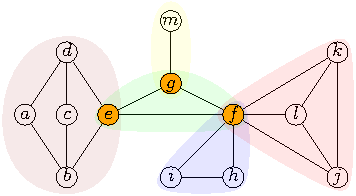
\includegraphics[width=0.4\textwidth]{bct_decomposed}
    }
    \hfill
    \subcaptionbox{Block-cut tree of a graph \label{fig:bidec:bctree}} {
        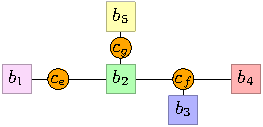
\includegraphics[width=0.4\textwidth]{bct_tree}
    }
    \hfill
    \subcaptionbox{Outer \(k\)-planar drawing of each component \label{fig:bidec:componnents_drawings}}{
        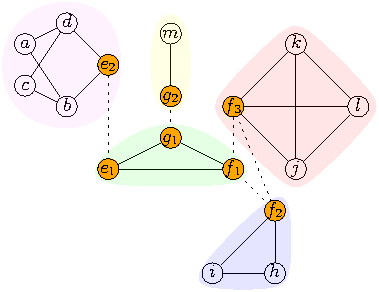
\includegraphics[width=0.4\textwidth]{bct_component_okp}
    }
    \hfill
    \subcaptionbox{
        Outer \(k\)-planar drawing of the original graph \label{fig:bidec:graph_drawing}} {
        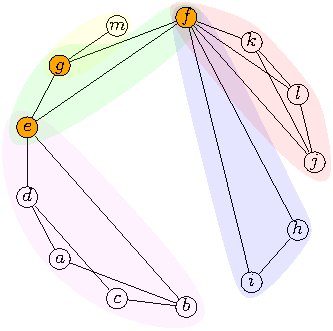
\includegraphics[width=0.4\textwidth]{bct_okp}
    }
    \caption{An example of a bicomponent decomposition}
\end{figure}

Due to the nature of bi-connectedness, after getting outer \(k\)-planar drawings of all biconnected components separately, we can combine them easily into an outer \(k\)-planar drawing of the whole graph. To be more specific, if some component does not admit an outer \(k\)-planar drawing, neither does the whole graph. Otherwise, if for all of them such a drawing exists, they can be merged by combining duplicates of each cut vertex see~\Cref{fig:bidec:componnents_drawings} and~\Cref{fig:bidec:graph_drawing}. This merging process does not introduce any additional edge crossings since both components are located on the outer face of each other. Moreover, as no new faces are created during this process (due to the acyclic structure of the block-cut tree), every vertex remains on the outer face of the graph during this process. Consequently, the resulting drawing of an original graph is outer \(k\)-planar, and it exists if and only if each biconnected component of the graph admits such a drawing.

In this work, we implemented this decomposition using the method \textsf{bi\-connec\-ted\_compo\-nents}\footnote{\url{https://www.boost.org/doc/libs/1_87_0/libs/graph/doc/biconnected_components.html}} from the Boost Graph Library~\cite{boost}. This function assigns an index of the bicomponent to each edge to which it belongs. Additionally, it provides a list of cut vertices. Afterwards, we copy each block as an independent graph and create mappings to translate new \emph{local} vertices back to their original identifiers. Finally, we construct a supergraph representing the structure of a block-cut tree wherein each node references a copied block alongside corresponding mapping or a cut vertex.

To construct a drawing of the whole graph, after performing the decomposition, we perform a depth-first search on the block-cut tree, recording the predecessor for each node upon discovery. Additionally, each time a block vertex is discovered, we use one of the methods described in~\Cref{sec:ILP-def,sec:SAT-def,sec:DP-def} to check whether the component admits an outer \(k\)-planar drawing and obtain it if so. Afterwards, we merge the new drawing with the already existing one by combining the common cut vertex if such exists. To be more specific, if the considered block is the first encountered one, its drawing is directly copied into a sequence that will form the final drawing. Otherwise, the block necessarily has a predecessor. Due to the structure of a tree, it is a cut node corresponding to a vertex that is shared with some other block. Due to how we traverse the tree, that other block has already been considered and thus added to a final drawing. As a result, the corresponding cut vertex is present in both global and local drawings. Since each drawing is represented as a cyclic sequence of vertices, we can rotate the local one so that the corresponding cut vertex appears as the first one in a sequence. Finally, we insert the local drawing starting from the second element into the global one immediately after the corresponding cut vertex.


\section{ILP-based algorithm}\label{sec:ILP-def}

The problem of recognising the outer \(k\)-planar graphs is NP-hard. This justifies the use of exponential-time methods to approach our problem. By doing so, we benefit from decade-long studies conducted for these problems that resulted in the development of extremely optimised algorithms for their solving. One of them is an Integer Linear Programming problem~(ILP). This problem asks to find a vector \(\mathbf{x}\) that optimises the linear objective \(\mathbf{c}^T\mathbf{x}\) subject to specific constraints \(\mathbf{Ax}\leqslant\mathbf{b}\). Additionally, some variables in the ILP problem are restricted to integer values. Since researchers have extensively studied the problem and developed efficient solvers, we decided to use their results to build an algorithm for recognising outer \(k\)-planar graphs. This section discusses the process we use to encode the recognition task as the ILP problem.

As an implementation of ILP solver, we used Gurobi Optimizer~\cite{gurobi} under the free academic licence. We chose it due to its outstanding performance demonstrated by \citeauthor{Gurobi-performance}~\cite{Gurobi-performance}.

To encode a recognition problem to an ILP, we have to represent its structure using variables and constraints. We start with a graph drawing, which is represented, as described above, as a sequence of vertices. For the ILP, we can encode it using the so-called \emph{ordering} variables, which indicate a relative order of two vertices. Specifically, for every pair of vertices \(u\) and \(v\), we create a binary variable \(a_{u, v}\) introducing ~\Cref{eq:ilp:con:order-var} as a constraint for the ILP problem. We interpret the value \(1\) as an indication of vertex \(u\) being located before vertex \(v\) and the value \(0\) as an indication of either \(v\) being located before \(u\) or \(u\) and \(v\) being the same vertex.

To ensure that these variables encode a valid sequence, we also have to enforce the transitivity. That is, for every ordered pair of distinct vertices \(u\) and \(w\), and every other vertex \(v\), if \(a_{u, v} = 1\) and \(a_{v, w} = 1\), meaning \(u\) is located before \(v\) and \(v\) is located before \(w\), then \(u\) must be located before \(w\), so the following should hold \(a_{u, w} = 1\). Including also the implication for the reversed order, we get:
\begin{align}
    a_{u, v} = 1 \land a_{v, w} = 1 \Longrightarrow a_{u, w} = 1 \label{eq:ilp:transitivity:uv:1}\\
    a_{u, v} = 0 \land a_{v, w} = 0 \Longrightarrow a_{u, w} = 0 \label{eq:ilp:transitivity:uv:0}
\end{align}
If we instead consider a pair \(w, u\) and the same vertex \(v\),  the constraints would look like follows:
\begin{align}
    a_{w, v} = 1 \land a_{v, u} = 1 \Longrightarrow a_{w, u} = 1 \label{eq:ilp:transitivity:vu:1} \\
    a_{w, v} = 0 \land a_{v, u} = 0 \Longrightarrow a_{w, u} = 0 \label{eq:ilp:transitivity:vu:0}
\end{align}
Note that for any distinct vertices \(x\) and \(y\) the equality \(a_{x, y} = 1 - a_{y, x}\) always holds, thus~\Cref{eq:ilp:transitivity:uv:1,eq:ilp:transitivity:vu:0} alike~\Cref{eq:ilp:transitivity:uv:0,eq:ilp:transitivity:vu:1} are equivalent. Consequently, it is enough to ensure only the first constraint as long as we do it for every ordered pair of vertices. Considering that the variables are binary, to limit \(a_{u, w}\) to \(1\) it is enough to impose a constraint \(a_{u, w} \geqslant \epsilon\) for any \(\epsilon \in (0;1]\). In a constraint for ILP, this \(\epsilon\) must be represented as a linear function of \(a_{u, v}\) and \(a_{v, w}\). The values of this function must lie in the half-interval \((0;1]\) if and only if both binary variables are \(1\). Using an expression \(a_{u, v} + a_{v, w} - 1\) for this leads to~\Cref{eq:ilp:con:transitivity} in the encoded ILP formulation below.

\begin{figure}[tbh]
    \centering
    \subfloat[][]{
\includegraphics[width=.3\textwidth]{edge_cross/uvst}\label{fig:edge_crossings:example-non-cross}} \hfill
    \subfloat[][]{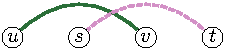
\includegraphics[width=.3\textwidth]{edge_cross/usvt}\label{fig:edge_crossings:example-cross}} \hfill
    \subfloat[][]{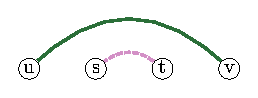
\includegraphics[width=.3\textwidth]{edge_cross/ustv}} \hfill
    \subfloat[][]{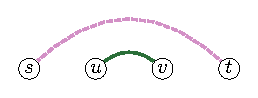
\includegraphics[width=.3\textwidth]{edge_cross/suvt}} \hfill
    \subfloat[][]{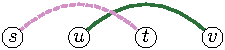
\includegraphics[width=.3\textwidth]{edge_cross/sutv}} \hfill
    \subfloat[][]{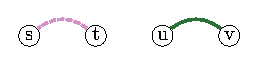
\includegraphics[width=.3\textwidth]{edge_cross/stuv}} \hfill

    \subfloat[][]{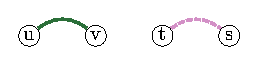
\includegraphics[width=.3\textwidth]{edge_cross/uvts}} \hfill
    \subfloat[][]{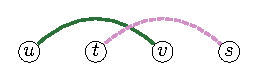
\includegraphics[width=.3\textwidth]{edge_cross/utvs}} \hfill
    \subfloat[][]{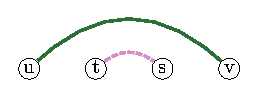
\includegraphics[width=.3\textwidth]{edge_cross/utsv}} \hfill
    \subfloat[][]{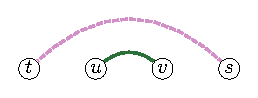
\includegraphics[width=.3\textwidth]{edge_cross/tuvs}} \hfill
    \subfloat[][]{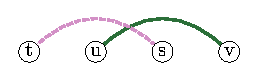
\includegraphics[width=.3\textwidth]{edge_cross/tusv}} \hfill
    \subfloat[][]{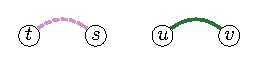
\includegraphics[width=.3\textwidth]{edge_cross/tsuv}} \hfill

    \subfloat[][]{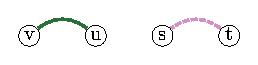
\includegraphics[width=.3\textwidth]{edge_cross/vust}} \hfill
    \subfloat[][]{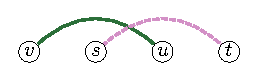
\includegraphics[width=.3\textwidth]{edge_cross/vsut}} \hfill
    \subfloat[][]{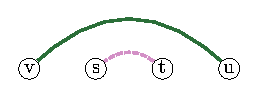
\includegraphics[width=.3\textwidth]{edge_cross/vstu}} \hfill
    \subfloat[][]{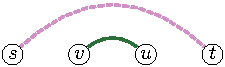
\includegraphics[width=.3\textwidth]{edge_cross/svut}} \hfill
    \subfloat[][]{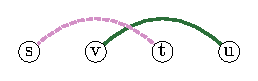
\includegraphics[width=.3\textwidth]{edge_cross/svtu}} \hfill
    \subfloat[][]{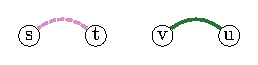
\includegraphics[width=.3\textwidth]{edge_cross/stvu}} \hfill

    \subfloat[][]{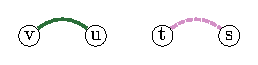
\includegraphics[width=.3\textwidth]{edge_cross/vuts}} \hfill
    \subfloat[][]{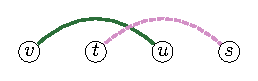
\includegraphics[width=.3\textwidth]{edge_cross/vtus}} \hfill
    \subfloat[][]{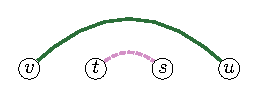
\includegraphics[width=.3\textwidth]{edge_cross/vtsu}} \hfill
    \subfloat[][]{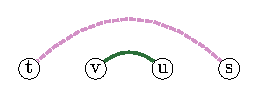
\includegraphics[width=.3\textwidth]{edge_cross/tvus}} \hfill
    \subfloat[][]{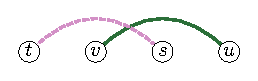
\includegraphics[width=.3\textwidth]{edge_cross/tvsu}} \hfill
    \subfloat[][]{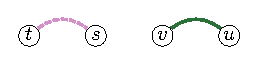
\includegraphics[width=.3\textwidth]{edge_cross/tsvu}}
    \caption{All \(24\) possible arrangements of the endpoints of two edges, only \(8\) of which result in an intersection; see the central column.}
    \label{fig:edge_crossings}
\end{figure}

The next step of the algorithm is to encode the intersections. To represent them, for every unordered pair of edges, \(uv\) and \(st\), we introduce a binary \emph{crossing} variable \(c_{uv, st}\), hence~\Cref{eq:ilp:con:cross-var} representing this constraint. The endpoints of the edges can be arranged in \(24\) different ways, among which only eight result in an intersection, as demonstrated in~\Cref{fig:edge_crossings}. To encode this, we must ensure that the value of the variable \(c_{uv, st}\) equals \(1\) if the corresponding ordering variables indicate one of these eight arrangements\footnote{As the objective of the program is to minimise the number of crossings, we do not constraint \(c_{uv, st}\) to \(0\) when \(uv\) and \(st\) do not cross, leaving this to the optimiser. Doing so, we simplify the problem by reducing the number of constraints for every pair of edges from \(24\) to \(8\).}. For example, considering the arrangement in~\Cref{fig:edge_crossings:example-cross}, we have to limit the value of \(c_{uv, st}\) to \(1\) if the endpoints are arranged in the order \(usvt\). This order of vertices is implied by the model if and only if each equivalence out of \(a_{u,s} = 1\), \(a_{s,v} = 1\) and \(a_{v,t} = 1\) holds. Thus, we can represent this limitation as follows:
\begin{align*}
    a_{u,s} = 1 \land a_{s,v} = 1 \land a_{v,t} = 1 \Longrightarrow c_{uv, st} = 1
\end{align*}
To transform this into a constraint for an ILP formulation, we can use the same logic as for encoding~\Cref{eq:ilp:transitivity:uv:1}, getting as a result~\Cref{eq:ilp:con:cross-example}. \Crefrange{eq:ilp:con:cross-begin}{eq:ilp:con:cross-end} are constructed analogously for the other seven intersecting arrangements.

Lastly, the algorithm has to encode each edge's crossing number and minimise the maximal value out of them. The crossing number of each edge can be easily represented as a sum of the corresponding crossing variables:
\begin{align}
    \label{eq:ilp:crossing-number}
    cr_{e_1} \leqslant \sum_{e_2 \in E(G)} c_{e1, e2}
\end{align}
However, as the maximum is not a linear function, constructing the objective function out of the per-edge crossing numbers is not as simple. To get around this limitation, we have to introduce a new continuous variable \(k\), which represents the crossing number of the whole graph \(G\). To ensure that, we have to bound \(k\) from below by the crossing number of each edge: \(k \geqslant cr_{e_1} \forall e_1 \in E(G)\). Combining this with~\Cref{eq:ilp:crossing-number}, we get~\Cref{eq:ilp:con:crossing-number} as a constraint for the ILP problem. As a result, minimising for \(k\) would give the desired result.

Combining everything together, we get the following formulation of the ILP problem:
\begin{align}
    \textbf{minimize}\quad&k  \label{eq:ilp:objective}\\
    \textbf{subject to}\quad
    &&a_{u, v} &\geqslant a_{u, v} + a_{v, w} - 1,&&\forall u, v, w \in V(G)  \label{eq:ilp:con:transitivity}\\
    &&c_{uv, st} &\geqslant a_{u,s} + a_{s,v} + a_{v,t} - 2,&&\forall uv, st \in E(G)  \label{eq:ilp:con:cross-example}\\
    &&c_{uv, st} &\geqslant a_{u,t} + a_{t,v} + a_{v,s} - 2,&&\forall uv, st \in E(G) \label{eq:ilp:con:cross-begin}\\
    &&c_{uv, st} &\geqslant a_{v,s} + a_{s,u} + a_{u,t} - 2,&&\forall uv, st \in E(G)\\
    &&c_{uv, st} &\geqslant a_{v,t} + a_{t,u} + a_{u,s} - 2,&&\forall uv, st \in E(G)\\
    &&c_{uv, st} &\geqslant a_{s,u} + a_{u,t} + a_{t,v} - 2,&&\forall uv, st \in E(G)\\
    &&c_{uv, st} &\geqslant a_{t,u} + a_{u,s} + a_{s,v} - 2,&&\forall uv, st \in E(G)\\
    &&c_{uv, st} &\geqslant a_{s,v} + a_{v,t} + a_{t,u} - 2,&&\forall uv, st \in E(G)\\
    &&c_{uv, st} &\geqslant a_{t,v} + a_{v,s} + a_{s,u} - 2,&&\forall uv, st \in E(G)  \label{eq:ilp:con:cross-end}\\
    &&k &\geqslant \sum_{st \in E(G)} c_{uv, st},&&\forall uv \in E(G)  \label{eq:ilp:con:crossing-number}\\
    &&c_{uv, st} &\in \{0, 1\},&&\forall uv, st \in E(G)  \label{eq:ilp:con:cross-var}\\
    &&a_{u, v} &\in \{0, 1\},&&\forall u, v \in V(G)  \label{eq:ilp:con:order-var}
\end{align}

To estimate the complexity of the formulation, we can calculate the number of constraints used in the encoding. So considering them in the order they are mentioned above, we have \(O(n^3) + 8\cdot O(m^2) + O(m) + O(m) + O(n) = O(n^3 + m^2)\) constraints, where \(n\) is the number of vertices and \(m\) is the number of edges in the input graph. Note that the size of the ILP formulation does not depend on the graph's local circular crossing number.

After encoding the problem as an ILP problem, as we described above, we run the solver. After optimisation, it returns assigned values for each variable used in the program. The variables of interest for us are ordering variables \(a_{u, v}\) and \(k\). The latter one indicates the minimal possible crossing number that is reported. The former one we use to reconstruct an outer \(k\)-planar drawing of the original graph. As the desired drawing is a sequence of vertices, we must order them. To do so, we can use the values of ordering variables to define the strict total order relation. We say that for two vertices \(u\) and \(v\) \(u < v\) if and only if \(a_{u, v}\) is assigned to \(1\). Due to the construction of these variables and transitivity constraints represented with~\Cref{eq:ilp:con:transitivity}, this order satisfies all requirements of the strict total order. Thus, it can sort the vertices, resulting in an outer \(k\)-planar drawing.


\section{SAT-based algorithm}\label{sec:SAT-def}

Another example of a thoroughly studied problem with an exponential-time solver is a Boolean Satisfiability problem~(SAT). As an input, the problem gets a boolean formula in a conjunctive normal form~(CNF). For the output, it asks for such an assignment of logic values \textsc{True} and \textsc{False} to the variables used in the input, such that the expression evaluates to \textsc{True}. This section discusses our process of encoding the recognition task into the SAT problem. To do so, we represent our problem as a boolean expression, which is satisfied if and only if the graph admits an outer \(k\)-planar drawing. As an implementation of SAT solver, we used kissat~\cite{kissat,kissat-library}. We chose it for our work as this solver is one of the best-performing ones~\cite{sat-competition}.

To encode the drawing, we use the ordering variables \(a_{u, v}\) we used in the ILP-based algorithm described in the~\Cref{sec:ILP-def} interpreting the value \(1\) as \textsc{True} and \(0\) as \textsc{False}. To encode the transitivity constraint, we follow the same logic, ending up with the same~\Cref{eq:ilp:transitivity:uv:1}. In terms of boolean algebra, this can be encoded as follows:
\begin{align*}
    a_{u, v} \land a_{v, w} \rightarrow a_{u, w}
\end{align*}
To transform this into CNF, we expand the implication and apply De Morgan's law, getting the first set of clauses in the SAT representation:
\begin{align}
    a_{u, v} \land a_{v, w} \rightarrow a_{u, w}
    &\equiv \overline{(a_{u, v} \land a_{v, w})} \lor a_{u, w} \nonumber \\
    &\equiv \overline{a_{u, v}} \lor \overline{a_{v, w}} \lor a_{u, w} \label{sat:trans}
\end{align}

To encode the edges' intersections, we also reuse crossing variables \(c_{uv, st}\) from the ILP-based algorithm. Similarly, we ensure that the variable is set to \textsc{True} if the endpoints of the corresponding edges are arranged in one of eight crossing patterns (see~\Cref{fig:edge_crossings}). This leads to eight sets of clauses, each of which contains ones representing one of these arrangements for all crossing variables. For example, for the arrangement from~\Cref{fig:edge_crossings:example-cross} the constraint for the variable \(c_{uv, st}\) can be encoded as follows:
\begin{align*}
    a_{u,s} \land a_{s,v} \land a_{v,t} \rightarrow c_{uv, st}
\end{align*}
To get a clause out of it, we expand the implication and apply De Morgan's law:
\begin{align}
    a_{u,s} \land a_{s,v} \land a_{v,t} \rightarrow c_{uv, st}
    & \equiv \overline{a_{u,s} \land a_{s,v} \land a_{v,t}} \lor c_{uv, st} \nonumber \\
    & \equiv \overline{a_{u,s}} \lor \overline{a_{s,v}} \lor \overline{a_{v,t}} \lor c_{uv, st} \label{sat:crossing-vars}
\end{align}

The last thing to encode is the limit of \(k\) intersections per edge. Unlike the ILP-based algorithm, we cannot add the corresponding variable. To impose this restriction, we ensure that no edges are crossed at least \(k+1\) times. For that, for each edge \(e_0\) and every set of \(k+1\) edges \(E = \{e_1, e_2, \dots, e_{k+1}\}\) we add a following clause to the boolean formula:
\begin{align}
    \overline{c_{e_0, e_1}} \lor \overline{c_{e_0, e_2}} \lor \cdots \lor \overline{c_{e_0, e_{k+1}}} \label{sat:cr-limit}
\end{align}
which evaluates to \textsc{True} if and only if at least one variable is set to \textsc{False}. By inserting this clause for every possible set \(E\), we ensure that no \(k+1\) edges cross the same edge. Thus, if the resulting boolean expression is satisfiable by some realisation of the variables, the values of ordering variables from this realisation would indicate an outer \(k\)-planar drawing.

Lastly we combine clauses from~\Cref{sat:trans} for all triplets of vertices \(u\), \(v\) and \(w\), with clauses from~\Cref{sat:crossing-vars} for all pairs of edges \(uv\) and \(st\), and with clauses from~\Cref{sat:cr-limit} for all edges \(e_0\) and all sets \(E\) of \(k+1\) edges. We combine the clauses using logical and operator (\(\land\)), as every single clause must be satisfied to graph to be outer \(k\)-planar. Then, we run the SAT solver using the resulting boolean expression as an input. If the solver fails to find a satisfiable instance, the algorithm halts, indicating that the graph is not outer \(k\)-planar. Otherwise, the algorithm halts returning the desired graph drawing. To reconstruct an outer \(k\)-planar drawing, similar to the ILP approach, we sort the vertices using the values of the ordering variables assigned by the solver to specify the order.

Unfortunately, unlike the algorithm based on ILP, this one does not solve the optimisation problem of finding the minimal possible \(k\). The resulting algorithm solves the decision problem~--~whether the graph admits an outer \(k\)-planar drawing or not. To transform this into an optimisation, we incrementally check each integer, starting from \(0\), until the boolean expression becomes satisfiable.

Finally, to estimate the complexity of the described formulation, we calculate the number of clauses in the Boolean expression. So by considering them in the order they are mentioned above, we get \(O(n^3) + O(m^2) + O(m^{k+2}) = O(n^3 + m^{k+2})\) clauses, where \(n\) is the number of vertices and \(m\) is number of edges in the graph. Unlike in the ILP-based algorithm, here, the size of the encoded problem grows exponentially in terms of \(k\), which makes this encoding more complex.


\section{Optimisations for ILP- and SAT-based algorithms}\label{sec:optimisations}

In both ILP- and SAT-based algorithms, for encoding the intersection of two edges \(uv\) and \(st\), we used binary variable \(c_{uv, st}\). However, despite \(24\) possible arrangements of edges' endpoints (see~\Cref{fig:edge_crossings}), we imposed only \(8\) constraints in each algorithm. Each of these constraints covers one of the arrangements that result in the intersection, leaving the rest \(16\) for the solver to optimise. This section discusses two ways we considered helping the solver optimise these variables.

The first optimisation is a simple extension of the same logic we applied for the intersecting arrangements. To ensure the correct values of crossing variables, we can impose all \(24\) constraints on each one. The first eight we described in the corresponding~\Cref{sec:ILP-def,sec:SAT-def}. The other \(16\) we construct in a similar way. For example, to construct a constraint for an arrangement in~\Cref{fig:edge_crossings:example-non-cross}, we have to encode the following:
\begin{gather*}
    a_{u,v} = 1 \land a_{v,s} = 1 \land a_{s,t} = 1 \Longrightarrow c_{uv, st} = 0
\end{gather*}

To represent it as a linear constraint for an ILP-based algorithm, we have to limit \(c_{uv, st}\) from above if all three variables are \(1\). We can do so with an equation \(3 - a_{u,v} - a_{v,s} - a_{s,t}\), resulting in a constraint:
\begin{gather*}
    c_{uv, st} \leqslant 3 - a_{u,v} - a_{v,s} - a_{s,t},\quad\forall uv, st \in E(G)
\end{gather*}

For a SAT-based algorithm, we can transform the implication in the similar way we did it for the clause from~\Cref{sat:crossing-vars}:
\begin{align*}
    a_{u,v} \land a_{v,s} \land a_{s,t} \rightarrow \overline{c_{uv, st}}
    & \equiv \overline{a_{u,v} \land a_{v,s} \land a_{s,t}} \lor \overline{c_{uv, st}} \\
    & \equiv \overline{a_{u,v}} \lor \overline{a_{v,s}} \lor \overline{a_{s,t}} \lor \overline{c_{uv, st}}
\end{align*}

By repeating these constraints for all non-crossing arrangements, we get the algorithms with exact crossing variables.

Another optimisation that we considered can be implemented only for an ILP-based algorithm. The primary problem caused by this inaccuracy in ILP formulation is that the variables' influence on the objective function is not direct. The crossing variables constrain another variable \(k\), which in turn affects the objective function, so it might be hard for an optimiser to estimate the effect of crossing variables accurately. With this optimisation, we help the solver by introducing a small direct influence on an objective function bypassing the intermediate variable \(k\). To do so, we include an extra term in the objective function from~\Cref{eq:ilp:objective}: \(\frac{\sum c_{e_1, e_2}}{|E|^2}\). By using \(|E|^2\) as a dominator in the fraction, we ensure that the value of the inserted term never exceeds \(1\) so that the optimiser would always prioritise decreasing \(k\) over this term. As a result, the optimised objective function for the ILP problem is:
\begin{gather*}
    k + \frac{\sum_{e_1, e_2 \in E(G)} c_{e_1, e_2}}{|E|^2}
\end{gather*}


\section{DP algorithm}\label{sec:DP-def}

The last algorithm we considered was introduced by \citeauthor{okp}~\cite{okp}. Unlike previously discussed ones, this algorithm was explicitly designed to solve the recognition problem. This method uses the approach of dynamic programming, where the solution for a problem is built based on solutions of similar but smaller problems. Thus, the final drawing of the graph is built incrementally each time for a larger part of the original graph.

The whole process can be divided into steps. Each one of them can be parameterised by three parameters. The first is a pair of vertices \(u\) and \(v\) that split a graph into two parts, denoted as a link. The next is a set \(R_{uv}\) of vertices lying to the right of the link. And lastly the set \(E_{uv} = \{e_1, e_2, \dots, e_l\}\) of \(l\) edges crossing the \(uv\) link from the right to the left side. To represent each step separately, we introduce a graph \(G_{uv, R_{uv}}\) which consists of vertices \(\{u, v\} \cup R_{uv}\) alongside all connecting edges from an original graph \(G\) with inserted vertices \(t_1, t_2, \dots, t_l\) connected to corresponding vertices by edges \(e_1, e_2, \dots, e_l\). We call a configuration on each step \emph{drawable} if exists an outer \(k\)-planar drawing of a corresponding graph \(G_{uv, R_{uv}}\) which cyclic order contains \((u, t_{\tau(1)}, t_{\tau(2)}, \dots, t_{\tau(l)}, v)\) as a consecutive subsequence for some permutation \(\tau\). On each step, the algorithm finds all possible permutations for which the configuration is drawable and stores them in the lookup table.

In the implementation of the algorithm, we first construct an index of all possible configurations. It allows us to simply iterate through it later without searching for the next configuration. Since, on each step, we try to draw a configuration using two smaller drawable ones, we group them by the size of the right part, guaranteeing that all smaller drawable configurations are already discovered at any point of the process. Unfortunately, it is unfeasible to consider all possible configurations due to the sheer number of them. For a graph with \(n\) vertices, there are \(\frac{n(n-1)}{2}\) links with \(2^{n-2}\) possible right sides each. As the link together with the right side uniquely determines the edges that cross the link, totally there are \(n(n-1)\cdot2^{n-3}\) possible configurations.

To significantly reduce the search space, the authors used the result of \citeauthor{triangulations}. They showed~\cite{triangulations} that there is a vertex \(w\) from the right side of any drawable configuration that splits it into two smaller \emph{narrow} configurations for which \(|E_{uw}| \leqslant k\) and \(|E_{vw}| \leqslant k\). By reversing their argument, we get that \(G_{uv, R_{uv}}\) admits an outer \(k\)-planar drawing if and only if we can combine it from two narrow drawable configurations. This allows us to limit the considered configurations only to narrow once, reducing their number to~\(2^{O(k)}m^{k+O(1)}\)~\cite[Lemma 15]{okp} instances.

Despite this optimisation, there is still a massive number of configurations. To minimise the memory consumption and make it feasible, we represent the right sides as binary masks stored as 64-bit integers. This decision limits the current implementation to graphs with at most 64 vertices. However, considering the complexity of the algorithm, we believe the graphs of bigger sizes would require an unreasonable amount of resources anyway\footnote{Potentially it is possible to develop a specified bitmask object which could handle any number of vertices by using multiple integers stored in an array.}.

To populate this index, we start by iterating over possible values for \(l\)\footnote{By iterating over this first, we ensure that it is easy to extend the index for \(k+1\) edges if the check for outer \(k\)-planarity is unsuccessful.}. For each choice of \(l\) and each link \(uv\), we consider an augmented graph \(H\) obtained by removing \(u\) and \(v\) from the original graph \(G\) alongside all connected edges. Then, we select exactly \(l\) edges from \(H\) to cross the link \(uv\). These edges further subdivide some connected components of \(H\) into connected subcomponents. Crucially, as these subcomponents do not contain edges that cross the link, each one of them must be located entirely on one side. Thus, finding all valid right sides for a given link means finding all valid black-white colourings of subcomponents, where white indicates belonging to the right and black to the left side. Consequently, each selected edge has to connect subcomponents of different colours, or in other words, the metagraph of \(H\) with subcomponents as vertices connected by selected edges has to be bipartite. After ensuring this holds, we construct all possible right sides for the selected link. As each connected bipartite graph can be coloured in exactly two ways, there are exactly \(2^d\) possible right sides, where \(d\) is the number of connected components in \(H\).

After constructing an index, we proceed to fill the lookup table. In there, for each configuration, we record all discovered sets of arrangements of \(E_{uv}\) that can appear in an outer \(k\)-planar drawing of \(G_{uv, R_{uv}}\) grouped by the link \(uv\) and the right side \(R_{uv}\). Each arrangement \(A_{uv}\) apart from a permutation \(\tau\) of edges in \(E_{uv}\) also contains a map \(f_{uv}:E_{uv}\rightarrow \mathbb{N}_+\) that matches each edge from \(E_{uv}\) with its number of intersections in the drawing of \(G_{uv, R_{uv}}\).

To fill the corresponding cell of the lookup table, we have to find all arrangements for which a specific configuration is drawable. We start by selecting a split vertex \(w\) that belongs to the right side \(R_{uv}\). For each \(w\), we iterate over all configurations with a link \(uw\) and a right side \(R_{uw}\) that is a subset of \(R_{uv}\). Additionally, we also consider a complementary configuration with a link \(vw\) and right side \(R_{vw} = R_{uv} \setminus (R_{uw} \cup \{w\})\). For each such pair of configurations, we iterate over all pairs of drawable arrangements \(A_{uw}\) and \(A_{vw}\) saved in the lookup table and search for all possible ways to combine them into an outer \(k\)-planar drawing of \(G_{uv, R_{uv}}\).

There is only one way to glue drawings of two configurations together. However, to form a valid drawing of \(G_{uv, R_{uv}}\), we also have to decide on the order of edges crossing the link \(uv\) represented by a permutation \(\tau_{uv}\). To ensure the correctness of the solution, we go through all possible ones. For each permutation, we check whether the resulting drawing is valid~--~each edge is crossed at most \(k\) times~--~and construct a mapping \(f_{uv}\) if so. To do that, we focus on an inner triangle consisting of three vertices \(u\), \(v\) and \(w\), and all the edges crossing at least one of the links \(uv\), \(uw\) and \(vw\). Additionally, we include edge \((u, v)\) if such exists. Crucially, to calculate all the intersections apart from the edges, we also need the order in which they enter the triangle. As sides of the triangle are exactly the links, this order is represented in corresponding permutations: \(\tau_{uw}\) from \(A_{uw}\), \(\tau_{vw}\) from \(A_{vw}\) and \(\tau_{uv}\) which is considered one by one. To represent the order in the triangle, we insert \(l_{uv}\) helper vertices between \(u\) and \(v\), given that \(l_{uv}\coloneq|E_{uv}|\). We treat them as endpoints of corresponding edges that enter the triangle by crossing the link \(uv\). Similarly, we insert vertices along the links \(uw\) and \(vw\). Importantly, each inserted vertex is an endpoint only for one edge, and along each link, they are ordered according to the corresponding permutations. By considering these vertices as edges' endpoints, we limit the view to the intersections created by the combination of two parts, ignoring those in \(R_{uw}\) and \(R_{vw}\). So, to get the crossing number for each edge, apart from the ones we count in the triangle, we also have to add those accounted by \(f_{uw}\) and \(f_{vw}\). If the crossing number of any edge exceeds \(k\), we discard the permutation \(\tau_{uv}\) and proceed to the next one. Otherwise, we extract the mapping \(f_{uv}\) and, together with the current permutation \(\tau_{uv}\), add it as a new arrangement to the lookup table.

If at any moment, the algorithm finds a drawable configuration with the link \(uv\) and right side \(R_{uv} = V(G)\setminus\{u, v\}\), it halts indicating that \(G\) is outer \(k\)-planar. In this case, the graph \(G_{uv, R_{uv}}\) is equivalent to the original graph \(G\) and admits an outer \(k\)-planar drawing. If, on the other hand, we reach the end of the index and do not find such a configuration, the algorithm halts, indicating that the graph is not outer \(k\)-planar.

In case of success, apart from a positive answer, we also have to return the graph drawing. There are multiple ways to accomplish this. One is to use a backtracking algorithm after finding the configuration to rediscover all smaller configurations with which the last one was built. Another approach is to store information on how each configuration was constructed alongside each arrangement. The latter trades the memory consumption required for additional information in each arrangement for the time required to perform backtracking. We used the second option in our implementation as it is much easier. Moreover, the bottleneck of the current implementation is running time and not memory. As additional information, we opted to store the drawing of the right side. To get this, we combine the drawings of two parts on each step, inserting the split vertex \(w\) between them. As a result, to get the drawing of \(G\) having the drawable configuration \(G_{uv, R_{uv}}\), it is enough to add vertex \(u\) at the start and vertex \(v\) at the end of the drawing stored alongside the arrangement \(A_{uv}\) in the lookup table.

Similar to the SAT-based algorithm from the~\Cref{sec:SAT-def}, this method only tests whether the graph admits an outer \(k\)-planar drawing or not for a fixed \(k\), so to find the minimal possible crossing number, we have to check each value incrementally.


\section{Interface of the implementation}

To have the ability to invoke the implemented algorithms for some specific graph, we designed a command-line interface. As an input, it receives a graph and a name of the algorithm the user wants to invoke. As an output, the user receives a local circular crossing number \(k\) of the passed graph alongside its circular drawing, where each edge is intersected at most \(k\) times. To communicate with a user, we use the Graphviz~\cite{graphviz} \textsc{DOT} language for both the graph and its drawing. We use this representation as it is easily interpretable by humans and computers.

Speaking more precise, the command-line interface has \(1\) required parameter~--~an undirected graph, represented as a string in Graphviz \textsc{DOT} language~--~and \(2\) optional arguments: method specifying one of the three implemented algorithms and output file specifying a path to file in which the graph's drawing should be saved. By default, the former holds the value corresponding to the ILP-based algorithm, and the latter holds an empty string, indicating that the drawing should not be saved anywhere. After running the algorithm, the tool will display the local circular crossing number and/or potential error messages.

\begin{figure}
    \centering
    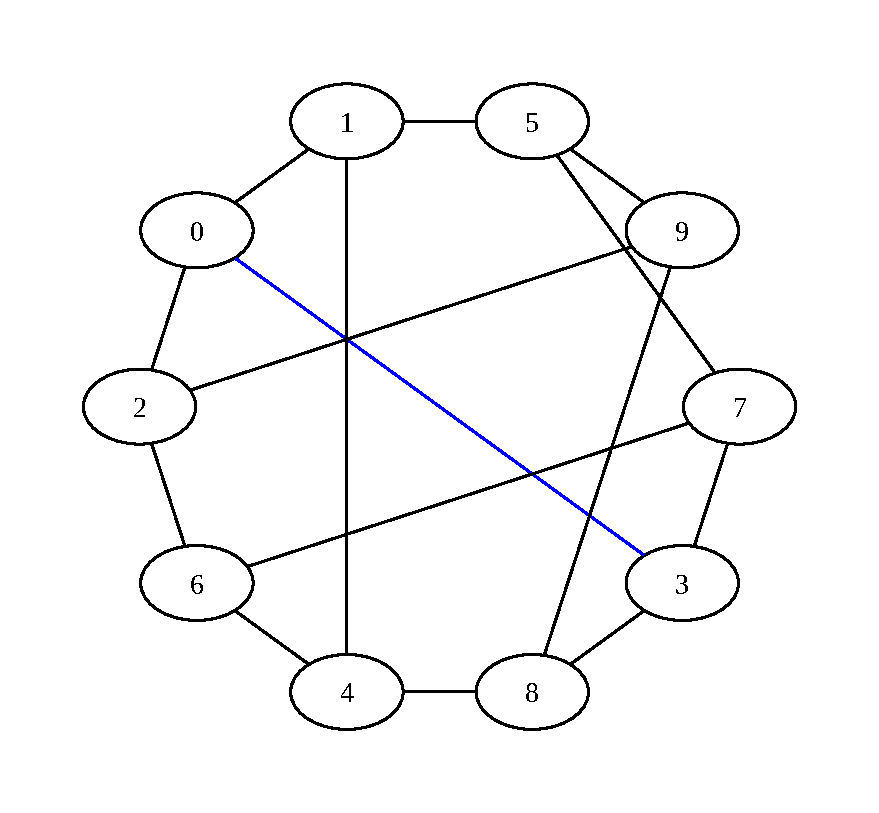
\includegraphics[width=.4\textwidth]{petersen}
    \caption{An example of the resulting drawing for the Petersen graph.}
    \label{fig:demo}
\end{figure}

To transform the returned drawing into a picture, we use the \textsf{neato} layout engine~\cite{neato}. An example of the drawing returned by an ILP-based algorithm for the Petersen graph is demonstrated in~\Cref{fig:demo}. Here, we use blue for edges that cross exactly \(k\) other edges, where \(k\) is the local circular crossing number.
